\chapter{Long-range electron correlation}\label{chap:vdw-methods}

{\sffamily This chapter presents a review of the state of the art of microscopic models of van der Waals interactions that have been applied beyond simple toy models and have a basis in the adiabatic-connection fluctuation--dissipation (ACFD) formula for the exchange-correlation energy.
While the reviewed methods are all prior works of other authors, the unified range-separation formalism based on the nonlocal polarizability, formal classification along the different approximations to the ACFD formula, and several re-derivations of existing methods are novel.
Most of the original and derived results in this chapter have been published in \citep{HermannCR17}.
}

\section{Range separation of electron correlation}\label{sec:range-separation}

The vdW force between atomic bodies held together by covalent, ionic, or metallic binding is always caused by the long-range electron correlation, but not all effects of the long-range correlation are considered to be a vdW force.
In metals, the electrons from the nonconducting bands are localized on atoms, which form nonuniform islands in the sea of approximately uniform electron density of the conducting electrons \citep{TaoPRB10}.
Here, the long-range correlation between the conducting electrons contributes to the metallic binding.
In nonmetals, however, all electrons are nonconducting, the electron density is nowhere uniform, and long-range correlation is mostly associated with vdW interactions.

The electronic structure within a single uniform subsystem differs qualitatively in many aspects from that in a nonuniform system.
In a uniform system, the exchange effects, the KS density response function, and the XC kernel decay only algebraically with distance (they are long-ranged) as a result of the conducting electrons, whereas they decay exponentially (they are short-ranged) in nonuniform systems~\cite{GePRB15}.
(The true density response function decays algebraically in both cases because of electron correlation.)
Correspondingly, semilocal and hybrid XC functionals capture both short-range and long-range part of the XC energy in uniform systems, but only the short-range part in the nonuniform systems.
The vdW interactions can be therefore associated with all long-range electron correlation except for that between conducting electrons within a single uniform subsystem, which is fortunately covered by semilocal and hybrid density functionals.
The nonuniform situations include interactions between conducting electrons in disjoint metallic bodies, interactions of conducting electrons with localized electrons, either in the same metallic body, or in other bodies, as well as all interactions between localized electrons.

The XC energy can be formally divided into a short-range (sr) and long-range (lr) part via the ACFD formula in~\eqref{eq:acfd-xc} by separating the double spatial integral into two parts using a range-separating function, $f$, which should decay at least exponentially fast,
\begin{equation}
\begin{gathered}
  \iint\mathrm d\mathbf r_1\mathrm d\mathbf r_2=\iint\mathrm d\mathbf r_1\mathrm d\mathbf r_2\big(1-f(\mathbf r_1,\mathbf r_2)\!\big)+\iint\mathrm d\mathbf r_1\mathrm d\mathbf r_2f(\mathbf r_1,\mathbf r_2)\equiv\iint_\text{sr}\mathrm d\mathbf r_1\mathrm d\mathbf r_2+\iint_\text{lr}\mathrm d\mathbf r_1\mathrm d\mathbf r_2 \\
  f(\mathbf r,\mathbf r)=0\qquad f(\mathbf r,\mathbf r+\mathbf R)=1-O(\exp(-R))
\end{gathered}
\end{equation}
Considering the range-separating function to be a functional of the density, $f\equiv f[n]$, it can be in principle always constructed exactly for a given short-range (or long-range) part.
The short-range part of the ACFD expression accounts for short-range density fluctuations interacting via the short-range part of the Coulomb operator, while the long-range part accounts for long-range fluctuations interacting via the long-range Coulomb operator.
The statements above about the XC energy in uniform and nonuniform systems can then be summarized in the following way,
\begin{equation}
  \underbracket[0pt][2.5ex]{\overbracket[0pt][2.55ex]{E_\text{xc}}^\text{uniform:}}_\text{nonuniform:}=\overbrace{\underbrace{E_\text{x,sr}+E_\text{c,sr}}_\text{semilocal/hybrid}+\underbrace{E_\text{x,lr}}_{\approx 0}+\underbrace{E_\text{c,lr}}_\text{vdW}}^\text{semilocal/hybrid}
\end{equation}
Of course, such a range separation is exact only in principle, because the association of a given XC functional with a particular range-separating function is unknown.

With the caveat about the uniform systems, the vdW interactions can then be associated with the long-range XC energy,
\begin{equation}
\begin{gathered}
  E_\text{xc,lr}=-\frac1{2\pi}\int_0^\infty\mathrm du\iint\mathrm d\mathbf r_1\mathrm d\mathbf r_2\int_0^1\mathrm d\lambda\,\chi(\mathbf r_1,\mathbf r_2,\mathrm iu;\lambda)v_\text{lr}(\mathbf r_1,\mathbf r_2) \\
  v_\text{lr}(\mathbf r,\mathbf r')=f(\mathbf r,\mathbf r')v(|\mathbf r-\mathbf r'|)
\end{gathered}
\label{eq:range-separation}
\end{equation}
In this setup, care must be taken about the potential double counting of the long-range XC energy in uniform systems from the semilocal or hybrid functionals and from the long-range ACFD formula.
This double-counting does not matter in situations when the result of a calculation is an energy difference, such as when calculating the adsorption energy of a molecule on a metal surface.
But it may pose a problem in other cases, for instance when investigating a lattice expansion of a metal.

The TD-DFT Dyson-like equation for the density response function in~\eqref{eq:dyson-td-dft} can be effectively range-separated by introducing some long-range effective Coulomb operator, $v_\text{eff}$, grouping the XC kernel (short-ranged in nonuniform systems) and the corresponding short-range Coulomb operator, $v-v_\text{eff}$, and averaging the resulting effective density response function, $\chi_\text{eff}$, over $\lambda$,
\begin{equation}
\begin{aligned}
  \chi^{-1}(\mathbf r,\mathbf r',u;\lambda)&=\chi^{-1}(\mathbf r,\mathbf r',u;0)-f_\text{xc}(\mathbf r,\mathbf r',u;\lambda)-\lambda\big(v(|\mathbf r-\mathbf r'|)-v_\text{eff}(\mathbf r,\mathbf r')\!\big)-\lambda v_\text{eff}(\mathbf r,\mathbf r') \\
  &\approx\chi^{-1}_\text{eff}(\mathbf r,\mathbf r',u)-\lambda v_\text{eff}(\mathbf r,\mathbf r')
\end{aligned}
\label{eq:dyson}
\end{equation}
Interpreting the response functions as tensors on the vector space of spatial functions, and using the shorthand multiplication notation for tensor composition, the full density response function can be expressed explicitly,
\begin{equation}
\begin{aligned}
  \textstyle\int_0^1\mathrm d\lambda\chi(u;\lambda)&=\textstyle\int_0^1\mathrm d\lambda\big(\chi_\text{eff}(u)+\chi_\text{eff}(u)\lambda v_\text{eff}\chi(u;\lambda)\!\big) \\
  &=\textstyle\int_0^1\mathrm d\lambda\big(\chi_\text{eff}(u)+\chi_\text{eff}(u)\lambda v_\text{eff}\chi_\text{eff}(u)+\chi_\text{eff}(u)\lambda v_\text{eff}\chi_\text{eff}(u)\lambda v_\text{eff}\chi(u;\lambda)\!\big) \\
  &=\sum_{n=0}^\infty\big(\textstyle\int_0^1\mathrm d\lambda\,\lambda^n\big)\chi_\text{eff}(u)\big(v_\text{eff}\chi_\text{eff}(u)\!\big)^n \\
  &=\sum_{n=0}^\infty\frac{1}{n+1}\big(\chi_\text{eff}(u)v_\text{eff}\big)^{n+1}v_\text{eff}^{-1} \\
  &=\ln\big(1-\chi_\text{eff}(u)v_\text{eff}\big)v_\text{eff}^{-1}
\end{aligned}
\end{equation}
The effective density response function, defined in this way, is guaranteed to be short-ranged in nonuniform systems.
The equivalent expressions can be written for the nonlocal dipole polarizability.

Plugging this expression to the long-range ACFD formula then gives the long-range XC energy in terms of the effective density response function and the two long-ranged Coulomb operators, $v_\text{eff}$ and $v_\text{lr}$,
\begin{equation}
\begin{aligned}
  E_\text{xc,lr}&=-\frac1{2\pi}\int_0^\infty\mathrm du\iint\mathrm d\mathbf r_1\mathrm d\mathbf r_2\big[\ln\big(1-\chi_\text{eff}(u)v_\text{eff}\big)v_\text{eff}^{-1}v_\text{lr}\big](\mathbf r_1,\mathbf r_2) \\
  &\equiv-\frac1{2\pi}\int_0^\infty\mathrm du\operatorname{Tr}_{\mathbf r}\Big(\ln\big(1-\chi_\text{eff}(u)v_\text{eff}\big)v_\text{eff}^{-1}v_\text{lr}\Big)
\end{aligned}
\end{equation}
The effective range of $v_\text{lr}$ is governed by the complementary range of the method for the short-range XC energy (typically a semilocal XC functional), whereas the range of $v_\text{eff}$ is controlled by the range of the model for the effective density response, discussed below.

\subsection{Static correlation}

In metals, strongly correlated materials, and spin-unpaired systems, the Coulomb interaction between electrons becomes at least as determining for the basic structure of the wave function as the kinetic energy.
This leads to the general failure of mean-field models such as the HF and semilocal KS-DFT approximations, except for metals and KS-DFT, in which the LDA-based XC functionals capture the electron correlation within uniform electron density effectively.
In spin-unpaired (open-shell) systems, this effect is often called static or left--right correlation.
Spin-unpaired systems typically result from breaking chemical bonds and separating the resulting fragments.
In such cases, a mean-field method can describe well the spin-paired unbroken system, but fails for the spin-unpaired separated fragments.
This might suggest that static correlation should be a part of the long-range correlation energy.

But consider the case of dissociating a hydrogen molecule in the (singlet) ground state into two hydrogen atoms.
The system of two separated atoms has zero total spin, and if one electron is measured on the left atom with some spin, the other will be certainly on the right atom because of Coulomb repulsion, and it will have the opposite spin.
The quantum states of the two hydrogen atoms are entangled, making them really a single quantum system, albeit noninteracting.
In a mean-field method, the probabilities of finding opposite-spin electrons at some points are uncorrelated, and there is 50\% chance that both electrons will be located on the same atom.
This underlying issue manifests differently in the HF and KS schemes.
In the HF approximation, the missing opposite-spin correlation in the wave function results in a spurious on-site repulsion.
In KS-DFT, on the other hand, the lack of correlation in the KS ground state is an expected part of the theory, resulting in two hydrogen atoms with mixed spin densities.
Current XC functionals then fail by giving a different XC energy for such mixed-spin hydrogen atoms than for a pure-spin hydrogen atom.
This demonstrates that the problem of static correlation in DFT is in fact a local problem that can be formulated on a single isolated hydrogen atom.
Alternatively, one can argue that the Coulomb operator in the ACFD formula goes to zero at large distances, whereas the static correlation persists at all distances, so it must be the short-range (on-site) structure of the (spin) density response function that determines the correct XC energy in systems with static correlation.
In any case, static correlation is part of the short-range XC energy, and the long-range correlation energy is indeed responsible solely for vdW interactions (except in uniform systems).

That being said, the incorrect treatment of static correlation can have a large effect on the response properties of the electronic system, and so the long-range correlation energy as well.
For instance, minimization of the total electronic energy with respect to semilocal and hybrid density functionals (which are incapable of treating static correlation) leads to electron densities that are far too diffuse and polarizable, which yields overestimated vdW interactions.
This issue, however, is present already in the isolated systems, and is independent of the long-range interaction between them.

\section{Local effective polarizability}\label{sec:local-pol}

This section argues that the formulation of the ACFD formula in terms of the nonlocal polarizability is a better starting point for developing approximate models than the formulation in terms of the density response function.
Expressing $\chi$ in terms of $\boldsymbol\alpha$, using the same integration-by-parts technique as when deriving the relationship between $\chi$ and $\boldsymbol\alpha$ in~\eqref{eq:alpha-chi}, and transferring the divergence operators on the Coulomb operator, the ACFD formula can be cast in terms of the nonlocal dipole polarizability,
\begin{equation}
\begin{gathered}
  E_\text{xc,lr}[\boldsymbol\alpha]=\frac1{2\pi}\int_0^\infty\mathrm du\iint\mathrm d\mathbf r_1\mathrm d\mathbf r_2\int_0^1\mathrm d\lambda\,\boldsymbol\alpha(\mathbf r_1,\mathbf r_2,\mathrm iu;\lambda)\mathbf T_\text{lr}(\mathbf r_1,\mathbf r_2) \\
  \mathbf T_\text{lr}(\mathbf r,\mathbf r')=\boldsymbol\nabla\otimes\boldsymbol\nabla' v_\text{lr}(\mathbf r,\mathbf r')
\end{gathered}
\end{equation}
Following the same procedure as with the density response function, this can be recast in terms of the effective polarizability,
\begin{equation}
\begin{aligned}
  E_\text{xc,lr}=\frac1{2\pi}\int_0^\infty\mathrm du\operatorname{Tr}_{\mathbf r}\Big(\ln\big(1+\boldsymbol\alpha_\text{eff}(u)\mathbf T_\text{eff}\big)\mathbf T_\text{eff}^{-1}\mathbf T_\text{lr}\Big)
\end{aligned}
  \label{eq:acfd-vdw}
\end{equation}

\begin{figure}
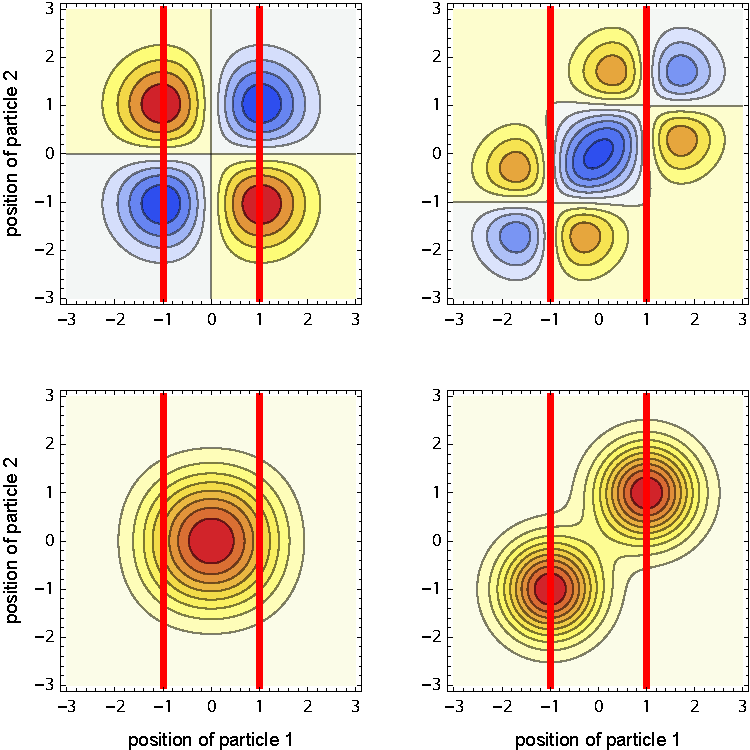
\includegraphics[center]{media/chi-vs-alpha}
\caption{\textbf{Density response function vs.\ dipole polarizability.}
Contour plots of model one-dimensional nonlocal (left) and local (right) responses encoded as the density response function (top), $\chi(x,y)$, and the dipole polarizability (bottom), $\alpha(x,y)$, defined in~\eqref{eq:model-responses}.
The red and blue colors correspond to positive and negative values.
The red lines denote the positions of the two responding Gaussian charge densities on the $x$-axis.
}\label{fig:chi-vs-alpha}
\end{figure}

There are three reasons why the effective-polarizability version of the ACFD formula turns out to be a good starting point for approximate models.
First, models of $\boldsymbol\alpha_\text{eff}$ can effectively capture all short-range XC effects, which modify the magnitude of the bare KS polarizability, without accounting for these effects explicitly via the Dyson equation.
Second, such models do not need to represent the short-range structure of the polarizability correctly, because it interacts only via the long-range dipole operators.
Third, the density response function has a complex nodal structure, as it describes depletion of the electron density at some points and its accumulation elsewhere.
In contrast, the corresponding polarizability is a rotation-free smooth vector field that encodes that underlying nodal structure implicitly in terms of its local behavior via the divergence operators in~\eqref{eq:alpha-chi}.
This is true even in the case of a long-ranged nonlocal density response function that is characteristic of uniform systems.
Therefore, the strength of the response is translated directly into the magnitude of the polarizability, whereas it is translated only indirectly into the magnitude of the gradient of the density response function.

For illustration, consider two one-dimensional (1D) Gaussian charge densities located at $\pm 1$ (crude model of atoms), and two model density response functions, one local, $\chi_\text{loc}$, the other nonlocal, $\chi_\text{nlc}$, (Figure~\ref{fig:chi-vs-alpha}),
\begin{equation}
\begin{gathered}
\chi_\text{nlc}(x,x')=-(\mathrm e^{-(x+1)^2}-\mathrm e^{-(x-1)^2})(\mathrm e^{-(x'+1)^2}-\mathrm e^{-(x'-1)^2}) \\
\chi_\text{loc}(x,x')=-(x+1)\mathrm e^{-(x+1)^2}(x'+1)\mathrm e^{-(x'+1)^2}-(x-1)\mathrm e^{-(x-1)^2}(x'-1)\mathrm e^{-(x'-1)^2}
\end{gathered}
\label{eq:model-responses}
\end{equation}
In one dimension, the dipole polarizability is a scalar, and uniquely determined by integrating over the density response function,
\begin{equation}
\alpha^\text{1D}(x,x')=\int_{-\infty}^x\mathrm dy\int_{-\infty}^{x'}\mathrm dy'\chi^\text{1D}(y,y')
\end{equation}
Even in these trivial models, the density response function changes sign around atoms, and has a nontrivial nodal structure, whereas the polarizability is positive everywhere.
Furthermore, the nonlocal density response translates into a polarizability that is still localized, but over a larger region spanning both atoms.
These observations are crucial for multipole expansions of both $\chi$ and $\boldsymbol\alpha$ discussed below.

The localized nature of the dipole polarizability combined with the insensitivity of the long-range ACFD formula to the short-range structure of the effective polarizability hints at the possibility of a relatively accurate local representation of $\boldsymbol\alpha_\text{eff}$, formally obtained by integrating over some neighborhood, $M(\mathbf r)$, around each point, $\mathbf r$,
\begin{equation}
  \boldsymbol\alpha_\text{eff}(\mathbf r,\mathbf r',u)\approx\delta(|\mathbf r-\mathbf r'|)\int_{M(\mathbf r)}\mathrm d\mathbf r''\boldsymbol\alpha_\text{eff}(\mathbf r,\mathbf r'',u)\equiv\delta(|\mathbf r-\mathbf r'|)\boldsymbol\alpha_\text{eff}(\mathbf r,u)
\end{equation}
Since $\alpha_\text{eff}(\mathbf r,u)$ depends on the properties of the system only in the near neighborhood of $\mathbf r$, good semilocal approximations to it can be constructed using local quantities such as the electron density, its gradient, or the KS kinetic energy density, in a similar manner that the hierarchy of semilocal XC functionals is built.
In nonuniform systems, the polarizability is localized only algebraically, the effective neighborhoods would need to be larger, and correspondingly, the range separation of the Dyson-like equation would need to be shifted towards larger separations.
On the other hand, in the case of a vdW interaction between a metal and a nonmetal, the long-range nonlocal electronic fluctuations in the former do not have any long-range counterpart in the latter, preventing any correlation on such length scales, and only relatively short-range fluctuations in the metal contribute to the vdW attraction.
For this reason, the local effective polarizability can effectively capture the true response even in such cases.

\subsection{Harmonic oscillator as a polarizability model}

The frequency dependence of the imaginary part of the density response function or dipole polarizability encodes the full optical (electromagnetic) spectrum.
This is equivalent to knowing the full energy spectrum of the corresponding Hamiltonian, which is a much harder problem than calculating the ground-state energy.
Accordingly, the ACFD formula contains the polarizability under the integral sign over all frequencies, and it is sufficient to model the spectrum only such that its sum-total is represented accurately.
This is done conveniently by modeling directly the imaginary-axis dependence of the polarizability, $\boldsymbol\alpha_\text{eff}(\mathbf r,\mathrm iu)$, which is a real-valued monotonically decreasing function, and must decay quadratically in the high-frequency limit.
These conditions are satisfied by a simple rational function (the simplest Padé approximant), specified by two parameters, $\boldsymbol\alpha(0)$ and $\omega$,
\begin{equation}
  \boldsymbol\alpha_\text{eff}(\mathbf r,\mathrm iu)\approx\frac{\boldsymbol\alpha_\text{eff}(\mathbf r,0)}{1+\frac{u^2}{\omega(\mathbf r)^2}}
\end{equation}
The interpretation of this formula is provided by a charged harmonic oscillator, for which it is the exact result.

Consider a particle with a charge, $q$, and mass, $m$, in a harmonic potential, $v_\text{ext}(\mathbf r)=m\omega^2/2$, and under a dissipative force, $-m\zeta\mathrm d\mathbf r/\mathrm dt$ (Lorentz oscillator).
The total polarizability of such a system can be expressed in a closed form,
\begin{equation}
  \alpha_\text{tot}^\text{LO}(u;\zeta)=\frac{q^2/m}{\omega^2-u^2+\mathrm i\zeta u}
  \label{eq:osc-pol}
\end{equation}
The electronic Hamiltonian without any interaction with the environment is nondissipative, and the corresponding oscillator model is recovered at the limit of $\zeta\rightarrow0$,
\begin{equation}
\begin{aligned}
  \lim_{\zeta\rightarrow 0}\alpha_\text{tot}^\text{LO}(u;\zeta)&=\frac{q^2/m}{\omega^2-u^2}+\frac\pi2\frac{q^2}{m\omega}\delta(u-\omega) \\
  \alpha_\text{tot}^\text{LO}(\mathrm iu;0)&=\frac{q^2/m\omega^2}{1+u^2/\omega^2}
\end{aligned}
\end{equation}
The same result is obtained using either a classical or quantum treatment.

\section{Classification of vdW methods}

\begin{figure}
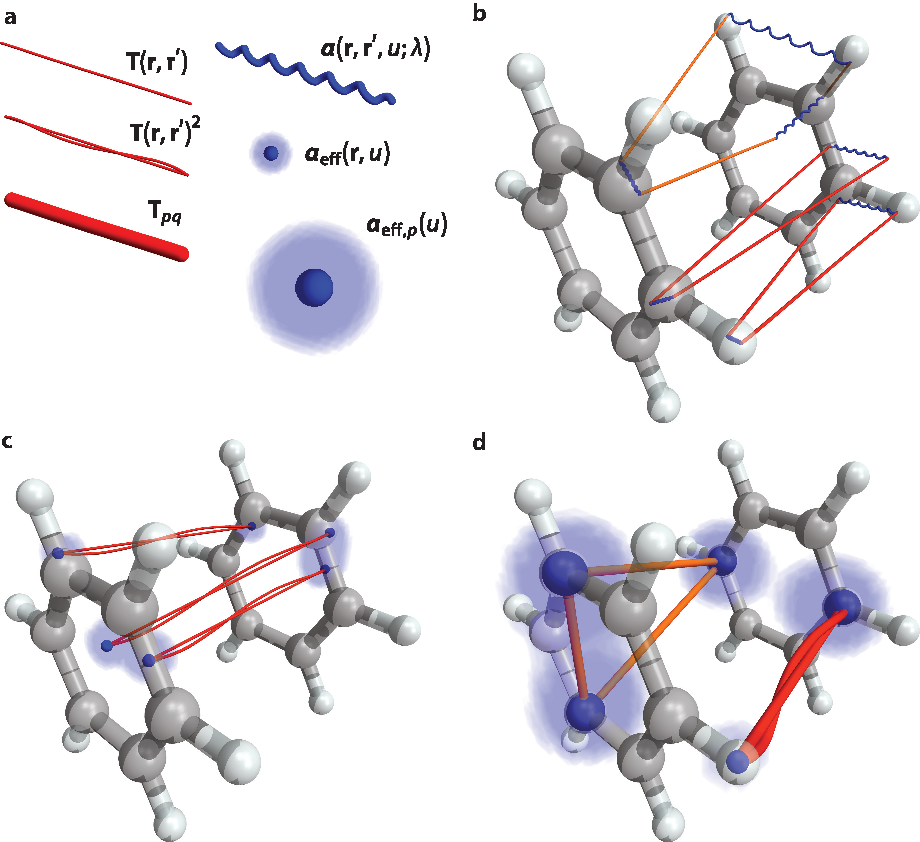
\includegraphics[center]{media/methods-diagrams}
\caption{\textbf{Coarse-graining and many-body expansion.}
Different kinds of approximations to the adiabatic-connection fluctuation--dissipation formula for the long-range exchange--correlation energy are shown on the ball-and-sticks model of the benzene dimer.
(\textbf a) Legend for the graphical representation of polarizabilities, $\boldsymbol\alpha$, and dipole operators, $\mathbf T$.
The clouds around the effective polarizability represent its effective spatial extent.
(\textbf b) The random-phase approximation is an ab-initio many-body method without coarse-graining that approximates the true coupling of the bare Kohn--Sham polarizability with a bare dipole operator.
The long-range part of the XC energy is formed by terms in which at least one of the dipole operators is long-ranged.
The red and orange colors denote second- and third-order terms, respectively.
(\textbf c) Nonlocal density functionals are second-order effective models without coarse-graining.
The polarizability is approximated locally.
(\textbf d) Many-body dispersion is a coarse-grained atomic model.
}\label{fig:diagrams}
\end{figure}

Most existing models of long-range correlation can be described in terms of various approximations to the range-separated effective-polarizability version of the ACFD formula in~\eqref{eq:acfd-vdw}.
One of them is the already discussed local representation of the effective polarizability.
Two other general and common approximations are spatial coarse-graining of the system and truncation of the infinite logarithm series, $\ln(1-x)=\sum_{n=1}x^n/n$.
The two types of approximations are illustrated in Figure~\ref{fig:diagrams}.

\subsection{Coarse-graining of continuous quantities}\label{sec:coarse-graining}

Given a set of functions, $w_p(\mathbf r)$, that partition a space into fragments, $\sum_p w_p(\mathbf r)\equiv1$, and respective centers of the fragments, $\mathbf R_p$, each spatial function or operator, such as the dipole polarizability, can be represented as a sum over the partitioned components, $\boldsymbol\alpha_{pq}$, which can be in turn expanded in the basis of solid harmonics (multipole expansion), $\alpha_{pq,ll'mm'}$, around the centers \citep{Stone13},
\begin{equation}
  \boldsymbol\alpha(\mathbf r,\mathbf r',u)=\sum_{pq}w_p(\mathbf r)w_q(\mathbf r')\boldsymbol\alpha(\mathbf r,\mathbf r',u)\equiv\sum_{pq}\boldsymbol\alpha_{pq}(\mathbf r,\mathbf r',u)\rightarrow\alpha_{pq,ll'mm'}
\end{equation}
(Here, $l$, $l'$ start from 1, because the expanded quantity is a tensor.
The corresponding expansion of the scalar density response fucntion, $\chi$, would start from $l=l'=0$.)
The dipole potential is expanded correspondingly.
Unlike the Fourier transformation, the multipole expansion is not invertible, but like the Fourier transformation, it introduces a correspondence between spatial integrals and infinite sums,
\begin{equation}
  \mathbf P(\mathbf r,u)=-\int\mathrm d\mathbf r'\boldsymbol\alpha(\mathbf r,\mathbf r',u)\mathbf E(\mathbf r',u)
  \ \Leftrightarrow\ 
  \mathbf P_{p,lm}(u)=-\sum_{q,l'm'}\alpha_{pq,ll'mm'}(u)E_{q,l'm'}
\end{equation}
The sums can be made implicit by arranging the multipole moments in vectors and matrices,
\begin{equation}
\begin{gathered}
  \boldsymbol\alpha=\begin{pmatrix}
    \boldsymbol\alpha_{pp} & \boldsymbol\alpha_{pQ} & \cdots \\
    \boldsymbol\alpha_{Qp} & \boldsymbol\alpha_{QQ} & \cdots \\
    \vdots & \vdots & \ddots
  \end{pmatrix}\\
  \boldsymbol\alpha_{pp}=\begin{pmatrix}
    \alpha_{11,11xx} & \alpha_{11,11xy} & \alpha_{11,11xz} & \alpha_{12,11xx} & \cdots \\
    \alpha_{11,11yx} & \alpha_{11,11yy} & \alpha_{11,11yz} & \alpha_{12,11yx} & \cdots \\
    \alpha_{11,11zx} & \alpha_{11,11zy} & \alpha_{11,11zz} & \alpha_{12,11zx} & \cdots \\
    \alpha_{21,11xx} & \alpha_{21,11xy} & \alpha_{21,11xz} & \alpha_{22,11xx} & \cdots \\
    \vdots & \vdots & \vdots & \vdots & \ddots
  \end{pmatrix}\qquad
\end{gathered}
\end{equation}
Under this notation, the long-range ACFD formula in~\eqref{eq:acfd-vdw} has exactly the same form, but the operators are infinite matrices instead of nonlocal functions, and the trace is not over space, but over the fragments and multipole moments,
\begin{equation}
\begin{aligned}
  E_\text{xc,lr}=\frac1{2\pi}\int_0^\infty\mathrm du\operatorname{Tr}_{p,lm}\Big(\ln\big(1+\boldsymbol\alpha_\text{eff}(u)\mathbf T_\text{eff}\big)\mathbf T_\text{eff}^{-1}\mathbf T_\text{lr}\Big)
\end{aligned}
  \label{eq:acfd-cg}
\end{equation}
The motivation for this multipole reformulation is that because both $\mathbf T_\text{eff}$ and $\mathbf T_\text{lr}$ are long-ranged and their moments decay increasingly faster for higher $l$'s, all the matrix multiplications (infinite sums) converge quickly and can be approximated well by finite sums.

The feasibility of the coarse-graining and multipole expansions is dictated by the choice of the fragments and the response properties of the system.
In a nonuniform system, the nonlocal effective polarizability is exponentially localized on atoms, and atom-centered fragments are a natural basis of a quickly converging multipole expansion.
In a uniform system, the effective polarizability is long-ranged, diffused, and there are no natural centers for the multipole expansion, leading to large higher moments and slow convergence or even divergence of the expansion.
In principle, this problem is mitigated in combination with the KS-DFT, because the long-range XC energy within the uniform systems is captured by the semilocal or hybrid functional, and the multipole convergence of the correlation energy due to interaction with a separate uniform or nonuniform system is helped by larger separations between the fragments.
But such an interplay is not well understood, and none of the coarse-grained models reviewed in this chapter take advantage of this cancellation.
In general, the complex interaction of the delocalized response of metals and localized response of nonmetals (insulators or molecules) is one of the hardest problems for general approximate models of the long-range electron correlation.
It has been treated in select systems by effective parametrization of the metallic response from experimental measurements of the dielectric function \citep{RuizPRL12}, but the lack of any general efficient model still hinders modeling of hybrid material interfaces.

\subsection{Truncation of many-body expansion}

The operator logarithm in~\eqref{eq:acfd-vdw} is defined as an infinite series, and writing it out explicitly in terms of individual orders leads to a many-body decomposition of the XC energy,
\begin{multline}
  E_\text{xc,lr}=
  \textstyle\frac1{2\pi}\int_0^\infty\mathrm du\operatorname{Tr}\big(\boldsymbol\alpha_\text{eff}(u)\mathbf T_\text{lr}\big)
  -\frac1{4\pi}\int_0^\infty\mathrm du\operatorname{Tr}\big(\boldsymbol\alpha_\text{eff}(u)\mathbf T_\text{eff}\boldsymbol\alpha_\text{eff}(u)\mathbf T_\text{lr}\big) \\
  \textstyle+\frac1{6\pi}\int_0^\infty\mathrm du\operatorname{Tr}\big(\boldsymbol\alpha_\text{eff}(u)\mathbf T_\text{eff}\boldsymbol\alpha_\text{eff}(u)\mathbf T_\text{eff}\boldsymbol\alpha_\text{eff}(u)\mathbf T_\text{lr}\big)
  -\ldots
\end{multline}
The name ``many-body'' is best motivated in the coarse-grained models where the individual terms correspond to interactions between increasing number of fragments (bodies).
(The order does not necessarily correspond to the number of bodies.
At fourth order, for instance, some terms are a back-and-forth interaction between two bodies.)
When constructed from the bare KS polarizability, the first term would evaluate to the long-range part of the exact exchange (plus higher-order exchange screening), which is negligible in nonuniform systems but can be relevant in uniform systems (where it would be typically covered by a semilocal XC functional).
With any local approximation for the effective polarizability, the first term evaluates exactly to zero.
The second term is the leading term for vdW interactions and the basis of all nonlocal correlation functionals and coarse-grained pairwise methods reviewed below.
The third term corresponds to the Axilrod--Teller--Muto (ATM) three-body potential \citep{AxilrodJCP43,MutoNS43} when coarse-grained to atoms.

When the $\boldsymbol\alpha_\text{eff}\mathbf T_\text{eff}$ term in the logarithm is small enough, the series converges quickly, and the logarithm can be approximated well by a truncated expansion.
While this is usually not the case for the total long-range XC energy of a system, $\mathbf T_\text{eff}$ is often small enough between the interacting subsystems, and if one is interested only in the interaction energy, the series can be often truncated already after the second order, because the higher-order terms cancel out.
However, this is not the case in general, especially in strongly polarizable systems, or in lower-dimensional systems where $\boldsymbol\alpha_\text{eff}\mathbf T_\text{eff}$ is highly anisotropic.
The degree of approximation made by truncating the infinite logarithm series is difficult to assess a priori, and Chapter~\ref{chap:pi-pi} shows an example of a system where the higher-order terms contribute substantially to interaction energies.

\subsection{Kohn--Sham response and random-phase approximation}\label{sec:rpa}

The approximations to the ACFD formula that are full many-body and not coarse-grained can be based based on the bare KS response.
Because the KS density response function can be calculated directly from the KS orbitals (eq.\ \ref{eq:adler-wiser}), these approximations are usually formulated and evaluated in the $\chi v$-representation rather than the $\boldsymbol\alpha\mathbf T$-representation.
Furthermore, because the bare response has a well-defined short-range structure, this construction allows the evaluation of the total XC energy, not only its long-range part, so the use of these methods goes far beyond long-range correlation energy.
Here, however, we discuss the methods mostly from the perspective of vdW interactions.

The simplest of these methods is the RPA, which translates into zero XC kernel in the formalism of the ACFD formula and TD-DFT~\cite{RenJMS12}.
This corresponds to setting the effective polarizability to the bare KS polarizability, and the effective dipole operator to the full dipole operator,
\begin{equation}
\begin{aligned}
  E_\text{c}^\text{RPA}=\frac1{2\pi}\int_0^\infty\mathrm du\operatorname{Tr}_{\mathbf r}\Big(\ln\big(1+\boldsymbol\alpha(u;\lambda=0)\mathbf T\big)-\boldsymbol\alpha(u;\lambda=0)\Big)
\end{aligned}
\end{equation}
In the $\chi v$-representation, the expression can be evaluated straightforwardly using the explicit expression for $\chi(u;\lambda=0)$~\cite{FurchePRB01}.

The omitted XC kernel is short-ranged in nonuniform systems, but its omission influences both short-range and long-range correlation energy, because the short-range XC effects in the polarizability eventually couple via the long-range dipole operator in the ACFD formula.
As a result, although RPA does not suffer from any systematic errors in the long-range correlation energies, the overall accuracy is often worse than that of the many effective models reviewed below \citep{OlsenPRB13a}.
This is further amplified in vdW systems in equilibrium geometries, where the short-range XC energy also contributes to the total interaction energy.
Attempts at improvement go both ways, replacing the short-range correlation energy with a better model than RPA, as well as improving the effective polarizability.

\citet{KurthPRB99} suggested to correct the short-range correlation energy from RPA with that from a semilocal XC functional, in what they called the RPA+ method.
Rather than explicitly range-separating the ACFD expression, RPA+ removes the RPA short-range part by subtracting correlation energy from a specially designed semilocal correlation functional, $E_\text{c}^\text{GGA@RPA}$, and reintroduces it back with standard semilocal functional, $E_\text{c}^\text{GGA}$.
\begin{equation}
  E_\text{c}^\text{RPA+}=E_\text{c}^\text{RPA}-E_\text{c}^\text{GGA@RPA}+E_\text{c}^\text{GGA}
\end{equation}
$E_\text{c}^\text{GGA@RPA}$ is constructed in a similar way as standard functionals, but its uniform part is parameterized to reproduce the RPA energy of the electron gas rather than the true energy.
In a later version, this was refined so that also the gradient correction satisfied the short-range behavior of RPA~\cite{YanPRB00}.
RPA+ attempts to fix the short-range correlation energy of RPA, but the long-range part is unchanged, so the vdW force remains the same, and it is only the interaction due to electron-density overlap, which occurs at equilibrium, that can be possibly improved.
Furthermore, the range separation in RPA+ is unsystematic in the sense that there is no guarantee that $E_\text{c}^\text{GGA@RPA}$ and $E_\text{c}^\text{GGA}$ have the same effective range.

\citep{ToulousePRA04} formulated a range-separated version of the KS scheme, in which the XC functional is designed from the beginning to treat only the short-range part of the electron correlation.
This leads to an alternative range separation of the ACFD formula, in which $\boldsymbol\alpha(\lambda)$ is not the polarizability of the wave function that minimizes $\langle\Psi|\hat T+\lambda\hat V|\Psi\rangle$, but rather of one that minimizes $\langle\Psi|\hat T+\lambda\hat V_\text{lr}|\Psi\rangle$ \citep{ToulousePRL09}.
In this scheme, the RPA of the Dyson-like equation results in a model in which the effective polarizability is still equal to the bare KS polarizability, like in normal RPA, but the effective dipole operator is only the long-range part of the full operator.
The underlying assumption then is that the dipole operator and the XC kernel partially cancel out at short range, giving a different estimate of the effective polarizability than normal RPA\@.
This is supported by numerical evidence on select small systems.
A similar scheme, proposed earlier by \citet{KohnPRL98}, also uses a range-separated version of the KS scheme, but instead of obtaining the true polarizability at the RPA level, $\chi(\lambda)$ is obtained for each $\lambda$ by explicitly perturbing the corresponding $\lambda$-scaled system with electric field.

A straightforward way to improve the RPA is to devise approximate XC kernels, which improves the short-range behavior of the polarizability, and hence both short-range and long-range correlation energies.
Extending the LDA to the time domain, the adiabatic LDA (ALDA) assumes that the XC kernel has no memory, leading to a frequency-independent local XC kernel,
\begin{equation}
\begin{aligned}
  f_\text{xc}^\text{ALDA}(\mathbf r,\mathbf r',t-t')&=\delta(t-t')\frac{\delta^2E_\text{xc}^\text{LDA}[n]}{\delta n(\mathbf r)\delta n(\mathbf r')}=\delta(t-t')\delta(\mathbf r-\mathbf r')\frac{\mathrm d^2\big(n\varepsilon_\text{xc}^\text{UEG}(n)\!\big)}{\mathrm d n^2}\bigg|_{n=n(\mathbf r')} \\
  f_\text{xc}^\text{ALDA}(\mathbf r,\mathbf r',u)&=\delta(\mathbf r-\mathbf r')\frac{\mathrm d^2\big(n\varepsilon_\text{xc}^\text{UEG}(n)\!\big)}{\mathrm d n^2}\bigg|_{n=n(\mathbf r')}
\end{aligned}
\end{equation}
Unlike LDA, which is exact for the uniform electron gas (UEG), ALDA does not give the true XC kernel of the UEG (which is nonlocal in both time and space), and violates several known properties of the true XC kernel.
Despite that, it is a useful approximation in TD-DFT calculations when one is interested only in a certain range of the frequency spectra.
Still, it turns out not to be a good approximation in the ACFD formula, where it give worse results than the absent XC kernel of the RPA \citep{LeinPRB00}.

\citet{OlsenPRB12} constructed a correction to ALDA by fixing its large-$\mathbf q$ (short-range) behavior in the UEG to better reproduce the known exact behavior.
Taking this renormalized ALDA (rALDA) kernel, transforming back to real space and using the mean density in two points as the corresponding uniform density, this procedure gives a universal XC kernel,
\begin{equation}
  f_\text{xc}^\text{rALDA}(\mathbf r,\mathbf r',u)=f_\text{xc}^\text{UEG}\big(|\mathbf r-\mathbf r'|;n=\tfrac12(n(\mathbf r)+n(\mathbf r')\!)\!\big)
\end{equation}
This construction is computationally no more demanding that RPA, but improves upon RPA in almost every case tested \citep{OlsenPRB13,OlsenPRL14}.
The rALDA XC kernel gives a more realistic short-range screening of the bare KS polarizability, resulting in more accurate long-range correlation energies and better description of vdW systems.

A different path towards improving the accuracy of RPA can be taken using the many-body perturbation (MBPT) theory.
This is possible because, as \citet{Gell-MannPR57} showed, yet another equivalent definition of RPA is via a certain subset of Feynman diagrams, the so-called ring diagrams.
Summing different subsets of the diagrams similar to those corresponding to RPA then leads to different RPA-like models and sometimes confusing terminology, when a certain modification of the XC kernel in RPA is equivalent to adding additional terms to the RPA XC energy that do not seem to be related to RPA \citep{ScuseriaJCP08,JansenJCP10,AngyanJCTC11}.

The second-order Møller--Plesset correlation energy (MP2) consists of the Coulomb direct and exchange terms, of which only the former is long-ranged.
In this context, RPA can be understood as the sum of all MP2-like direct terms (ring diagrams) in the infinite MBPT expansion.
Similarly, the MP2 exchange can be renormalized by replacing one of the Coulomb interactions with the RPA sequence of ring diagrams, leading to the second-order screen exchange (SOSEX).
Furthermore, unlike in the Møller--Plesset perturbation theory, where the first order is guaranteed to be zero, single-electron excitations contribute to the XC energy in the MBPT based on KS orbitals.
Combining RPA, SOSEX and RPA-renormalized single-excitation correction then results in the renormalized second-order perturbation theory (rPT2) \citep{RenPRL11,RenPRB13}.
Although the MP2 exchange term is short-ranged, the renormalization in SOSEX is long-ranged, and the long-range correlation energy of rPT2 is different from that of RPA\@.
The combined improvements of the short-range and long-range XC energy in rPT2 compared to RPA lead to improved accuracy in vdW binding energies.

\subsection{Nonlocal density functionals}\label{sec:vdwdf}

The models of long-range correlation energy reviewed in this section are in the class of approximations to the ACFD formula that truncate the many-body expansion at second order, but do not do any spatial coarse-graining.
This leads to XC functionals that are characterized by nonlocal dependence of the XC energy density on the electron density via some nonlocal kernel, $\Phi$,
\begin{equation}
  E_\text{c,lr}^\text{nl-df}=\frac12\int\mathrm d\mathbf r\mathrm d\mathbf r'n(\mathbf r)n(\mathbf r')\Phi[n](\mathbf r,\mathbf r')=\int\mathrm d\mathbf r\,n(\mathbf r)\int\mathrm d\mathbf r'\tfrac12 n(\mathbf r')\Phi[n](\mathbf r,\mathbf r')
  \label{eq:nldf}
\end{equation}

The derivation of~\eqref{eq:nldf} from the ACFD formula for the XC energy starts with truncating the logarithm expansion at second order,
\begin{equation}
  E_\text{xc,lr}\approx
  \frac1{2\pi}\int_0^\infty\mathrm du\operatorname{Tr}_{\mathbf r,\mathbb R^3}\big(\boldsymbol\alpha_\text{eff}(u)\mathbf T_\text{lr}-\tfrac12\boldsymbol\alpha_\text{eff}(u)\mathbf T_\text{eff}\boldsymbol\alpha_\text{eff}(u)\mathbf T_\text{lr}\big)
\end{equation}
Here, $\operatorname{Tr}_{\mathbb R^3}$ denotes the trace over the three Cartesian vector components.
In the next step, the effective polarizability is approximated with a local isotropic polarizability,
\begin{equation}
  \boldsymbol\alpha_\text{eff}(\mathbf r,\mathbf r',u)\approx\mathbf I\alpha_\text{eff}(\mathbf r,u)\delta(\mathbf r-\mathbf r')
\end{equation}
This results in the first-order term being zero, which means that such a functional cannot capture any exchange energy, which is intentional, since the nonlocal functionals are designed to capture only the long-range correlation energy.
The locality of the effective polarizabilities reduces two of the four integrals in the second-order term, and the isotropy allows to take the polarizabilities out of the trace,
\begin{equation}
\begin{aligned}
  E_\text{c,lr}&\approx
  -\frac1{4\pi}\int_0^\infty\mathrm du\iint\mathrm d\mathbf r\mathrm d\mathbf r'\operatorname{Tr}_{\mathbb R^3}\big(\alpha_\text{eff}(\mathbf r,u)\mathbf T_\text{eff}(\mathbf r,\mathbf r')\alpha_\text{eff}(\mathbf r',u)\mathbf T_\text{lr}(\mathbf r',\mathbf r)\!\big) \\
  &=-\frac1{4\pi}\int_0^\infty\mathrm du\iint\mathrm d\mathbf r\mathrm d\mathbf r'\alpha_\text{eff}(\mathbf r,u)\alpha_\text{eff}(\mathbf r',u)\operatorname{Tr}_{\mathbb R^3}\big(-\mathbf T_\text{eff}(\mathbf r,\mathbf r')\mathbf T_\text{lr}(\mathbf r,\mathbf r')\!\big) \\
\end{aligned}
  \label{eq:acfd-nlc}
\end{equation}
Both $\mathbf T_\text{eff}$ and $\mathbf T_\text{lr}$ go to the bare dipole operator for large distances, and the trace can be rewritten in terms of a range-separating function, $f$,
\begin{equation}
\operatorname{Tr}_{\mathbb R^3}\big(-\mathbf T_\text{eff}(\mathbf r,\mathbf r')\mathbf T_\text{lr}(\mathbf r,\mathbf r')\!\big)\equiv f(\mathbf r,\mathbf r')\frac6{|\mathbf r-\mathbf r'|^6}
\label{eq:r6-func}
\end{equation}
This is the origin of the $1/R^6$ dependence of the pairwise vdW force.

A general form of the local effective polarizability used in many models is obtained from the polarizability of a harmonic oscillator by setting the ratio of the charge and mass to that of an electron, $q/m=1$, and substituting the electron density for the charge,
\begin{equation}
  \alpha_\text{tot}^\text{HO}(\mathrm iu)=\frac{q^2/m}{\omega^2+u^2}
  \quad\longrightarrow\quad
  \alpha_\text{eff}[n](\mathbf r,\mathrm iu)=\frac{n(\mathbf r)}{\omega^2_\text{eff}[n](\mathbf r)+u^2}
  \label{eq:local-eff-pol}
\end{equation}
Besides the obvious reason of modeling electrons, the charge--mass ratio of one is motivated by the $f$-sum rule for an electronic system that dictates that $\alpha_\text{tot}(\mathrm iu)\rightarrow N/u^2$ ($N$ is the number of electrons), which the form above automatically satisfies.
(Strictly speaking, this is not necessary, because the rule does not need to be satisfied in any local form, and furthermore, the local effective polarizability is not supposed to integrate to the total polarizability without any long-range coupling.
However, the local form is a straightforward way to satisfy the global rule.)
The local effective resonance frequency, $\omega^2_\text{eff}$, can be in general any functional of the electron density, but is often approximated locally.

Combining~\eqref{eq:local-eff-pol},~\eqref{eq:r6-func}, and~\eqref{eq:acfd-nlc}, the approximated ACFD formula can be recast in the form of a nonlocal density functional, where the nonlocal kernel is a functional of the effective resonance frequency and the (unspecified) range-separating function,
\begin{equation}
  E_\text{c,lr}\approx
  \frac12\iint\mathrm d\mathbf r\mathrm d\mathbf r'\,n(\mathbf r)n(\mathbf r')\bigg(-\frac3{\pi}\int_0^\infty\mathrm du\frac1{\omega^2[n](\mathbf r)+u^2}\frac1{\omega^2[n](\mathbf r')+u^2}\frac{f(\mathbf r,\mathbf r')}{|\mathbf r-\mathbf r'|^6}\bigg)
  \label{eq:acfd-kernel}
\end{equation}
The asymptotic behavior of the long-range correlation energy calculated in this way is fully specified by $\omega_\text{eff}$.

The first general functional of this form, referred to simply as the vdW density functional (vdW-DF), was developed by \citet{DionPRL04} as a culmination of a program set up by \citet*{AnderssonPRL96}.
The program was followed along a different branch by \citet{HultPRL96,HultPRB99}, but this effort did not result in a general functional of only the electron density.
Although the derivation of the vdW-DF starts from the ACFD formula, it follows quite a different direction than the framework in this chapter, and most of the approximations along the way are done in reciprocal space, until everything is transformed back to real space in the end.
However, the final result can still be cast in the form of~\eqref{eq:acfd-kernel}.

The effective resonance frequency in the vdW-DF is constructed from a GGA-type XC energy density,
\begin{equation}
\omega^2_\text{vdW-DF}[n](\mathbf r)=4\pi^2\varepsilon_\text{xc}^\text{vdW-DF}[n]^4
  =4\pi^2\left(
      \varepsilon_\text{xc}^\text{UEG}(n)
      +A\left\lvert\frac{\mathbf\nabla n}{n^\frac76}\right\rvert^2
      \right)^4
\end{equation}
The first equality is motivated by using $\omega^2_\text{eff}$ to calculate the XC energy of a slowly varying electron gas via the ACFD formula.
The particular choice of the semilocal approximation to the XC energy density is rather arbitrary and completely independent of the semilocal functional potentially used to complete the vdW-DF at short range.
The value of the numerical parameter $A$ can be derived in different ways using different first-principles arguments, leading to substantially different values and results for vdW binding energies~\cite{LeePRB10}.

A serious disadvantage of the vdW-DF in light of other long-range correlation models is that its range-separating function is fixed by the underlying theory.
Because of the construction in the reciprocal space, the parameter $A$ appears both in the effective resonance frequency and the range-separating function.
Since the asymptotic behavior of any nonlocal functional depends only on $\omega_\text{eff}$, not the range-separating function, the parameter $A$ is essentially fixed, and there is no remaining freedom in the range-separating function that could be adjusted for a particular choice of a short-range semilocal functional in a full KS-DFT calculation.

The form of the range-separating function is complex due to the reciprocal-space formulation, but there are two underlying physical motivations for it.
When the two oscillators given by the resonance frequencies $\omega_\text{eff}$ are close to each other such that their ground-state wave functions would overlap, the underlying model does not work anymore, the corresponding part of the XC energy must be covered by the semilocal functional, and the dipole coupling must be damped.
This is effectively achieved by increasing the resonance frequency as $k^2$ in the reciprocal space.
The second damping mechanism is that the nonlocal functional must evaluate to zero for the uniform electron gas, whose long-range correlation energy is already covered by a semilocal or a hybrid functional.
This forces the range-separating function to negative values at short range, to counterbalance the attractive contribution from the long range.

The complex form of the vdW-DF was gradually simplified by \citeauthor{VydrovJCP09}.
In the vdW-DF-09~\cite{VydrovJCP09}, the range-separating mechanism was constructed independently of the effective resonance, making the nonlocal functional adaptable to any semilocal or hybrid functional, which also resulted in improved accuracy for vdW binding energies.
Furthermore, the local resonance frequency was somewhat modified,
\begin{equation}
  \omega^2_\text{vdW-DF-09}[n](\mathbf r)=(4\pi)^2\underbrace{\frac{4^3\pi^2}{3^6}}_{\doteq 0.87}\left(
      \varepsilon_\text{x}^\text{UEG}(n)
      +B\left\lvert\frac{\mathbf\nabla n}{n^\frac76}\right\rvert^2
      \right)^4
  \label{eq:vdw-df-09}
\end{equation}

Further simplification was achieved in the VV09 functional, which used a substantially different form of $\omega_\text{eff}$,
\begin{equation}
  \omega^2_\text{VV09}[n](\mathbf r)=\frac{4\pi}3n(\mathbf r)+C\frac{|\boldsymbol\nabla n|^4}{n^4}
  \label{eq:vv-pol}
\end{equation}
Here, $4\pi n$ is the resonance frequency of the macroscopic (small-$\mathbf q$ limit) plasmon fluctuations of the uniform electron gas.
The factor of $1/3$ comes from the Clausius--Mossotti relation between the microscopic local polarizability and the macroscopic dielectric function.
The density-gradient term is a local model of a band gap obtained from considering the behavior of the electron density in the density tail of a finite system.
The range-separating mechanism of VV09 is still constructed in reciprocal space.

The final attempt at a simplified formulation of the vdW-DF, named VV10, was constructed entirely in real space~\cite{VydrovJCP10a}.
Both the resonance frequency and range-separating function of~\eqref{eq:acfd-kernel} have a simple form in VV10.
The former is the same as in VV09, and the latter is constructed using the same mechanism of reduced polarizabilities of overlapped oscillators as in the original vdW-DF, but in real space,
\begin{equation}
  f_\text{VV10}(\mathbf r,\mathbf r')=\frac{\alpha_\text{eff}(\mathbf r,\mathrm iu;\omega=\omega_\text{VV09}+Dn^\frac13/|\mathbf r-\mathbf r'|^2)\alpha_\text{eff}(\mathbf r',\mathrm iu;\omega=\omega_\text{VV09}+Dn^\frac13/|\mathbf r-\mathbf r'|^2)}{\alpha_\text{eff}(\mathbf r',\mathrm iu;\omega=\omega_\text{VV09})\alpha_\text{eff}(\mathbf r',\mathrm iu;\omega=\omega_\text{VV09})}
  \label{eq:damping-vv10}
\end{equation}
As $1/|\mathbf r-\mathbf r'|^2$ grows at short distances, the effective resonance frequency of the local oscillators increases, reducing their polarizability.
The parameter $D$ is used to adjust the range of this mechanism.

\subsection{Pairwise interatomic models}\label{sec:pairwise}

The oldest approaches to fix the missing long-range electron correlation in HF or semilocal KS-DFT calculations are of the interatomic pairwise form,
\begin{equation}
  E_\text{c,lr}\approx-\frac12\sum_{pq}C_{6,pq}
  \frac{f(\mathbf R_p,\mathbf R_q)}{|\mathbf R_p-\mathbf R_q|^6}
  \label{eq:pairwise}
\end{equation}
Here, $f$ is some range-separating (damping) function, $\mathbf R_q$ are the atom coordinates, and the so-called dispersion coefficients, $C_{6,pq}$, determine the asymptotic interaction between two atoms.
This type of interatomic potential has origin in empirical force fields dating back to the Lennard--Jones potential, even before it was clear that the correct leading term of the vdW force is $1/R^6$.
In the context of electronic-structure methods, it was first used by~\citet{HepburnCPL75} to correct interaction curves of rare-gas dimers from HF calculations.
This approach was later extended to molecules and KS-DFT calculations, and the $C_6$ coefficients were extended to a wider range of systems \citep{HalgrenJACS92,MooijJPCA99,ElstnerJCP01,WuJCP02}.
\citet{GrimmeJCC04} then presented a parametrization of $C_6$ and $f$, termed DFT-D (`D' for dispersion), that could in principle be applied to any molecule or solid, in combination with any XC functional.
This marked a start of routine addition of the long-range correlation energy to semilocal KS-DFT calculations.

The pairwise interatomic model of~\eqref{eq:pairwise} can be obtained as a coarse-grained truncated approximation to the ACFD formula.
The derivation follows the same course of second-order truncation and local approximation to the effective polarizability as nonlocal vdW XC functionals, but starting from the coarse-grained multipole-expanded ACFD formula in~\eqref{eq:acfd-cg},
\begin{equation}
  E_\text{c,lr}\approx
  \frac1{4\pi}\int_0^\infty\mathrm du\operatorname{Tr}_{p,lm}\big(\boldsymbol\alpha_\text{eff}(\mathrm iu)\mathbf T_\text{eff}\boldsymbol\alpha_\text{eff}(\mathrm iu)\mathbf T_\text{lr}\big)
\end{equation}
Here, the trace is over multipole moments and fragments, which are chosen to be atoms in most cases.
(In this context, the formal definition of an atom in a molecule is given by some partition function.)
Approximating the local effective polarizability as isotropic, $\alpha_{\text{eff},pll'mm'}=\delta_{ll'}\delta_{mm'}\alpha_{\text{eff},pl}$, the formula is reduced as in the case of nonlocal vdW XC functionals,
\begin{gather}
\begin{aligned}
  E_\text{c,lr}&\approx
  \frac1{4\pi}\int_0^\infty\mathrm du\sum_{pq}\sum_{ll'}\alpha_{\text{eff},pl}(\mathrm iu)\alpha_{\text{eff},ql'}(\mathrm iu)\big[\operatorname{Tr}_m(\mathbf T_\text{eff}\mathbf T_\text{lr})\big]_{pq,ll'} \\
  &=-\frac12\sum_{pq}\sum_{ll'}\left(\frac{K_{ll'}}{2\pi}\int_0^\infty\mathrm du\,\alpha_{\text{eff},pl}(\mathrm iu)\alpha_{\text{eff},ql'}(\mathrm iu)\right)\frac{f_{ll'}(\mathbf R_p,\mathbf R_q)}{|\mathbf R_p-\mathbf R_q|^{2+2l+2l'}} \\
  &\equiv-\frac12\sum_{pq}\sum_{ll'}C_{2+2l+2l',pq}\frac{f_{ll'}(\mathbf R_p,\mathbf R_q)}{|\mathbf R_p-\mathbf R_q|^{2+2l+2l'}}
\end{aligned}\label{eq:pairwise-mult} \\
K_{ll'}=\lim_{\mathbf R\rightarrow\infty}\frac{\sum_m T_{ll'mm}(\mathbf R)}{|\mathbf R|^{2+2l+2l'}}
\end{gather}
The standard pairwise formula of~\eqref{eq:pairwise} is recovered by keeping only the lowest dipole--dipole term ($l=l'=1$, $K_{11}=6$), where the expression for the corresponding dispersion coefficient is called the Casimir--Polder integral,
\begin{equation}
  C_{6,pq}=\frac3\pi\int_0^\infty\mathrm du\,\alpha_{\text{eff},p1}(\mathrm iu)\alpha_{\text{eff},q1}(\mathrm iu)
\end{equation}

Some pairwise methods are formulated directly in terms of the dispersion coefficients, not the underlying polarizabilities, in which case approximate combination rules for calculating unknown heteronuclear coefficients from known homonuclear coefficients are useful.
Such rules can be derived from the Casimir--Polder integral using some model polarizability.
An often used rule is obtained from the harmonic-oscillator model,
\begin{equation}
\begin{aligned}
  C_{6,pq}^\text{HO}&=\frac3\pi\int_0^\infty\mathrm du\frac{\alpha_p(0)\omega_p^2}{\omega_p^2+u^2}\frac{\alpha_q(0)\omega_q^2}{\omega_q^2+u^2}=\frac{3\alpha_p(0)\alpha_q(0)\omega_p\omega_q}{2(\omega_p+\omega_q)} \\
  &=\frac{2C_{6,pp}C_{6,qq}}{C_{6,pp}\frac{\alpha_q(0)}{\alpha_p(0)}+C_{6,qq}\frac{\alpha_p(0)}{\alpha_q(0)}}
\end{aligned}
\label{eq:comb-rule}
\end{equation}
Using the single-pole polarizability of the harmonic oscillator in situations where the true spectrum is more complex, such as in the equation above, is called the \citet{UnsoldZP27} approximation.

The models of Grimme are different from the rest reviewed in this section in that they are formulated only in terms of the geometry of a molecule, $\{\mathbf R_p\}$, not the electron density.
This makes them straightforwardly useful even for empirical short-range electronic models that do not produce any electronic density, but at the same time, it makes it much harder to achieve truly general models, because the electron density encodes much useful information about the system.

The first version of DFT-D used fixed homonuclear $C_6$ coefficients, the combination of~\eqref{eq:comb-rule} with all polarizability ratios set to 1, and a range-separating function constructed from vdW radii that did not go to 1 in infinity~\cite{GrimmeJCC04}.
The second version was a numerical reparametrization of the first one with a changed combination rule, which set the polarizability ratios equal to those of the $C_6$ coefficients~\cite{GrimmeJCC06}.
In the first and second version, the atomic $C_6$ coefficients do not depend on the molecular environment, which is a crude approximation.
The third version was an improvement in several regards~\cite{GrimmeJCP10}.
The range separation was modified to obey the correct asymptotic behavior.
An elementary dependence of the $C_6$ coefficients on the environment was included via geometrical factors estimating the coordination number of an atom.
The dipole--quadrupole term ($l=1$, $l'=2$) from~\eqref{eq:pairwise-mult} was included, and a three-atom correction was suggested, which is the third-order triple-dipole term in the logarithm expansion of the coarse-grained ACFD formula.
The corresponding dispersion coefficients, $C_8$ and $C_9$, are obtained by combination rules similar to those for the $C_6$ coefficient.

Soon after the first version of DFT-D and in stark contrast to it, \citet{BeckeJCP05b} developed a method to calculate $C_6$ coefficients from first principles, using an approximation to the polarizability based on the dipole moment of the XC hole of the HF model, the exchange-hold dipole method (XDM).
Their initial derivation was rather heuristic, with a wrong prefactor, but the final result can be in fact obtained directly from the Casimir--Polder integral using the fluctuation--dissipation theorem for the density response function of~\eqref{eq:fluctuation-dissipation} and the Unsöld approximation:
\begin{equation}
\begin{aligned}
  C_6&=\frac3\pi\int_0^\infty\mathrm du\alpha_\text{tot}(\mathrm iu)^2
  \approx\frac3\pi\int_0^\infty\mathrm du\left(\frac{\alpha_\text{tot}(0)}{1+u^2/\omega^2}\right)^2
  =\frac34\alpha_\text{tot}(0)^2\omega \\
  &=\tfrac12\alpha_\text{tot}(0)\frac3\pi\int_0^\infty\mathrm du\frac{\alpha_\text{tot}(0)}{1+u^2/\omega^2}
  =\tfrac12\alpha_\text{tot}(0)\frac3\pi\int_0^\infty\mathrm du\alpha_\text{tot}(\mathrm iu) \\
  &=\tfrac12\alpha_\text{tot}(0)\frac1\pi\int_0^\infty\mathrm du\operatorname{Tr}_{\mathbb R^3}\big(\boldsymbol\alpha_\text{tot}(\mathrm iu)\!\big) \\
  &=\tfrac12\alpha_\text{tot}(0)\frac1\pi\int_0^\infty\mathrm du\iint\mathrm d\mathbf r\mathrm d\mathbf r'\operatorname{Tr}_{\mathbb R^3}\big(\boldsymbol\alpha(\mathbf r,\mathbf r',\mathrm iu)\!\big) \\
  &=\tfrac12\alpha_\text{tot}(0)\iint\mathrm d\mathbf r\mathrm d\mathbf r'\operatorname{Tr}_{\mathbb R^3}\big(-\mathbf r\otimes\mathbf r'{\textstyle\frac1\pi\int_0^\infty}\chi(\mathbf r,\mathbf r',\mathrm iu)\!\big) \\
  &=\tfrac12\alpha_\text{tot}(0)\iint\mathrm d\mathbf r\mathrm d\mathbf r'\,\mathbf r\cdot\mathbf r'n(\mathbf r)\big(n_\text{xc}(\mathbf r,\mathbf r')+\delta(\mathbf r-\mathbf r')\!\big) \\
  &=\tfrac12\alpha_\text{tot}(0)\int\mathrm d\mathbf r\,\left(\mathbf rn(\mathbf r)\cdot\int\mathrm d\mathbf r'\,\mathbf r'\big(n_\text{xc}(\mathbf r,\mathbf r')+\delta(\mathbf r-\mathbf r')\!\big)\!\right) \\
  &\equiv\tfrac12\alpha_\text{tot}(0)\int\mathrm d\mathbf r\,\mathbf d_n(\mathbf r)\cdot\mathbf d_\text{xc}(\mathbf r)
\end{aligned}
\end{equation}
Here, the $C_6$ coefficient is expressed in terms of the static polarizability and the correlation between the local dipole moment of the total density and of the XC hole with its reference electron.
This expression provides accurate $C_6$ coefficients when provided with accurate correlated XC holes, but fails short of good accuracy when evaluated with the approximate XC hole from the HF model~\cite{AngyanJCP07}.
The XDM uses a slightly modified expression that autocorrelates the XC hole dipole moment,
\begin{equation}
  C_6\approx\tfrac12\alpha_\text{tot}(0)\int\mathrm d\mathbf r\,\mathbf d_\text{xc}(\mathbf r)\cdot\mathbf d_\text{xc}(\mathbf r)
\end{equation}
This version works remarkably well with the HF XC hole, but the reasons for this unexpected accuracy are not well understood~\cite{AngyanJCP07,HesselmannJCP09,AyersJMC09}.
A semilocal approximation to the XC hole by \citet{BeckePRA89} works as well as that from the HF model, and with the additional benefit of reduced computational complexity~\cite{BeckeJCP05a}.

To formulate a general interatomic pairwise method, the dipole moment of the XC hole is coarse-grained using the partitioning scheme devised by \citet{HirshfeldTCA77}.
In this scheme, the atomic partition functions, $w_p$, are constructed from radially averaged electron densities of isolated atoms, $n^\text{free}$,
\begin{equation}
  w^\text{Hirsh}_p(\mathbf r)=
  \frac{n^\text{free}_p(|\mathbf r-\mathbf R_p|)}
  {\sum_q n^\text{free}_q(|\mathbf r-\mathbf R_q|)}
  \label{eq:hirshfeld}
\end{equation}
The corresponding static dipole polarizabilities of the atomic fragments are calculated from free-atom dipole polarizabilities, assuming that they scale linearly with the Hirshfeld measure of a volume (Hirshfeld volume),
\begin{gather}
  \alpha_{p1}(0)=\alpha_{p1}^\text{free}(0)\frac{V^\text{Hirsh}_p[n]}{V^\text{Hirsh}_p[n^\text{free}]} \\
  V_p^\text{Hirsh}[n]=\int\mathrm d\mathbf r\,n(\mathbf r)w^\text{Hirsh}_p(\mathbf r)|\mathbf r-\mathbf R_p|^3
  \label{eq:hirshfeld-vol}
\end{gather}
The fragment $C_6$ coefficients are then calculated from the fragment polarizabilities and coarse-grained XC hole dipole moment,
\begin{equation}
  C_{6,pp}^\text{XDM}=\tfrac12\alpha_{p1}(0)\int\mathrm d\mathbf r\,w_p(\mathbf r)\mathbf d_\text{xc}(\mathbf r)\cdot\mathbf d_\text{xc}(\mathbf r)
\end{equation}
The harmonic-oscillator combination rule is used to get the rest of the $C_6$ coefficients.
The XDM can be extended to higher-multipole dispersion coefficients by calculating higher multipole moments of the XC hole polarization around each atomic center~\cite{BeckeJCP06,JohnsonJCP06}.

The XDM dispersion coefficients were paired with two distinct empirical suggestions for the range-separating function, one based on the ratio of approximate short-range and long-range correlation energies, the other on the vdW radii~\cite{BeckeJCP07},
\begin{align}
f_{11}^\text{XDM1}(\mathbf R_p,\mathbf R_q)&=\left(1+A\left(
  \frac{C_{6,pq}/|\mathbf R_p-\mathbf R_q|^6}
{E_{\text{c},p}^\text{free}+E_{\text{c},q}^\text{free}}\right)\right)^{-1} \\
f_{11}^\text{XDM2}(\mathbf R_p,\mathbf R_q)&=\left(1+A\left(\frac{R_{\text{vdW},p}+R_{\text{vdW},q}+B}{|\mathbf R_p-\mathbf R_q|}\right)^6\right)^{-1}
\end{align}
Here, $E_{\text{c},p}^\text{free}$ is the correlation energy of a free atom calculated with some semilocal correlation functional.

A simple yet accurate interatomic pairwise method was developed by \citet{TkatchenkoPRL09} (TS), who extended the free-atom scaling approach to all the atomic parameters, including the $C_6$ coefficients and the vdW radii, and thus formulating the calculation of interatomic pairwise vdW interactions into a true density functional.
Assuming that the excitation energies of the atoms are independent of the volume, the Unsöld approximation and the Casimir--Polder integral dictate that the $C_6$ coefficients scale with the second power of the Hirshfeld volume ratio,
\begin{equation}
  C_{6,pq}=C_{6,pq}^\text{free}\left(\frac{V^\text{Hirsh}_p[n]}{V^\text{Hirsh}_p[n^\text{free}]}\right)^2 \\
\label{eq:TS}
\end{equation}
The free-atom reference values may not be the most effective choice in metals and some solids, whose electron density is often substantially different from the superposition of free-atom densities.
\citet{ZhangPRL11} and \citet{RuizPRL12} used an adapted TS method, where the reference values are obtained from bulk macroscopic dielectric constant.
The TS method uses a logistic function as a range-separating function, with the free-atom vdW radii naturally scaled by the cubic root of the Hirshfeld-volume ratio,
\begin{equation}
  \label{eq:damping-ts}
  f_{11}^\text{TS}(\mathbf R_p,\mathbf R_q)=\left(1
    +\exp\left[
      -A\left(B\frac{|\mathbf R_p-\mathbf R_q|}{R_{\text{vdw},p}+R_{\text{vdw},q}}-1\right)
    \right]\right)^{-1}
\end{equation}

\citet{SatoJCP09,SatoJCP10} developed an atomic pairwise method based on the local effective polarizability functional from the vdW-DF-09 nonlocal functional.
Their local response dispersion (LRD) method is an explicit realization of the coarse-graining approach outlined in Section~\ref{sec:coarse-graining}.
A system is described by the local effective polarizability given by the harmonic-oscillator formula with the resonance frequency from~\eqref{eq:vdw-df-09}.
The atomic fragments are defined using the partitioning functions from the scheme by \citet{BeckeJCP88}, which is most often used to define atomic radial grids in KS-DFT calculations, but here it is used as an alternative to the Hirshfeld partitioning.
The partitioned polarizability is used to calculate a coarse-grained representation of the system via multipole expansion and Casimir--Polder integrals up to the $C_{10}$ coefficient.
The LRD method uses yet another range-separating function, parametrized by the polarizabilities in place of the vdW radii,
\begin{equation}
  f_{11}^\text{LRD}(\mathbf R_p,\mathbf R_q)
  =\exp\left(
    -\left(
      \frac
        {|\mathbf R_p-\mathbf R_q|}
        {A\big(\sqrt[3]{\alpha_{\text{eff},p}}+\sqrt[3]{\alpha_{\text{eff},q}}\big)+B}
    \right)^6
  \right)
\end{equation}

\citet{SilvestrelliPRL08} formulated a pairwise method in which the coarse-grained fragments are not atoms, but Wannier functions (WFs)~\cite{MarzariRMP12}.
Wannier functions are any set of localized one-electron wave functions that in principle form a complete basis.
In finite molecular systems, they are called Boys orbitals.
The Wannier functions of conducting and nonconducting electrons are localized algebraically and exponentially, respectively.
In the vdW-WF method, each WF is approximated with a single spherically symmetric exponential function that has the same width (second central moment) as the true WF\@.
The polarizability of the approximate WF is calculated with the polarizability functional of \citet*{AnderssonPRL96} (ALL),
\begin{equation}
  \alpha_{\text{eff},p}(\mathrm iu)
  =\int_{\mathbf r\in\Omega_A}
  \mathrm d\mathbf r\frac{n_p(\mathbf r)}{4\pi n_p(\mathbf r)+u^2},\quad
    \Omega_A=\{\mathbf r:|\mathbf\nabla n_p(\mathbf r)|<kn_p(\mathbf r)^\frac76\}
\end{equation}
Here, $n_p$ is the electron density of the WF and $k$ is a nonempirical constant.
The $C_6$ coefficients between the WFs are calculated from the Casimir--Polder integral, and the range-separating function is the same as in the TS method, with vdW radii of the WFs defined via an electron density cutoff~\cite{SilvestrelliJCP09}.
The vdW-WF scheme has two theoretical shortcomings: first, the partitioning of the total electron density is only approximate because of the use of the approximate WFs, and second, the ALL polarizability functional was designed for the total electron density, not one-electron densities.

Coarse-grained methods in which the fragment polarizabilities and $C_6$ coefficients are calculated directly, rather than obtained by explicit partitioning of some continuous quantity, may be sensitive to a particular choice of the partitioning scheme.
This motivated a series of modified Hirshfeld partitioning schemes that should capture better the redistribution of the electron density in a molecule with respect to free atoms.
\citet{SteinmannJCTC10,SteinmannJCTC11} adapted the XDM to use the self-consistent Hirshfeld scheme, which gives a more consistent description of ionic systems~\cite{BultinckJCP07}.
\citet{BuckoJCTC13,BuckoJCP14} did the same with the TS method.
The self-consistent Hirshfeld partitioning uses the same stockholder formula in~\eqref{eq:hirshfeld} as the original scheme, but the reference densities are generalized and depend recursively on the partitioning, leading to equations that need to be solved iteratively~\cite{VerstraelenJCTC12}.
A common form of the generalized reference densities, used in the modified XDM and TS methods, is a linear combination of free-atom and free-ion densities that maintains the charge of the Hirshfeld-partitioned atomic density.
This scheme is complicated by the instability of many isolated anions, which requires addition of auxiliary negative charges, making the partitioning somewhat arbitrary.

\subsection{Many-body dispersion framework}\label{sec:mbd}

The fourth and final class of approximations to the ACFD formula covers nontruncated coarse-grained models.
A common theme of all such models is to interpret the Unsöld approximation with its single resonance frequency literally, and model a real molecular system as a collection of coupled charged oscillators.
The corresponding Hamiltonian describes a system of distinguishable particles characterized by a charge, $q_i$, and a mass, $m_i$, each having its own harmonic potential defined by the resonance frequency, $\omega_i$, and a center, $\mathbf R_i$, interacting via the Coulomb force,
\begin{multline}
  \hat H_\text{osc}=\sum_i\frac{\mathbf{\hat p}_i^2}2+\sum_i\frac12 m_i\omega_i^2|\mathbf{\hat r}_i-\mathbf R_i|^2 \\
  +\sum_{i<j}q_i q_j\left(
    \frac1{|\mathbf{\hat r}_i-\mathbf{\hat r}_j|}
    -\frac1{|\mathbf{\hat r}_i-\mathbf R_j|}
    -\frac1{|\mathbf R_i-\mathbf{\hat r}_j|}
    +\frac1{|\mathbf R_i-\mathbf R_j|}
  \right)
\end{multline}
The centers of the harmonic potentials additionally host a compensating charge of the opposite sign.
If the centers are the same as those of the atoms, this Hamiltonian can be interpreted as a very crude approximation to the electronic Hamiltonian, in which all electrons of individual atoms are described by distinguishable psuedoelectrons that move in an effective potential which is the combined result of the nuclear potential and the mean field of the electrons.
In particular, any exchange effects and hence charge transfer and delocalization are scrapped.
Expanding the Coulomb operator in a multipole series and keeping only the dipole term results in dipole-coupled oscillator Hamiltonian,
\begin{equation}
  \hat H_\text{dosc}=\sum_i\frac{\mathbf{\hat p}_i^2}2+\sum_i\frac12 m_i\omega_i^2|\mathbf{\hat r}_i-\mathbf R_i|^2+\sum_{i<j}q_i q_j(\mathbf{\hat r}_i-\mathbf R_i)\mathbf T(\mathbf R_j-\mathbf R_i)(\mathbf{\hat r}_j-\mathbf R_j)
  \label{eq:mbd}
\end{equation}

A useful property of this Hamiltonian is that it can be solved exactly by coordinate transformation.
Introducing mass-scaled coordinates, $\hat{\boldsymbol\xi}_i=\sqrt{m_i}(\mathbf{\hat r}_i-\mathbf R_i)$, $\hat{\boldsymbol\xi}=(\hat{\boldsymbol\xi}_1\hat{\boldsymbol\xi}_2\ldots)$, using the expression for the polarizability of a charged harmonic oscillator in~\eqref{eq:osc-pol}, and the fact that the kinetic-energy operator is invariant with respect to unitary transformations, the dipole-coupled Hamiltonian can be transformed into uncoupled quasi oscillators,
\begin{equation}
\begin{aligned}
  \hat H_\text{dosc}&=\sum_i\frac{\mathbf{\hat p}_i^2}2+\sum_i\frac12\omega_i^2\hat{\boldsymbol\xi}_i^2+\frac12\sum_{ij}\omega_i\omega_j\sqrt{\alpha_i(0)\alpha_j(0)}\hat{\boldsymbol\xi}_i\mathbf T_{ij}\hat{\boldsymbol\xi}_j \\
  &\equiv\sum_i\frac{\mathbf{\hat p}_i^2}2+\frac12\hat{\boldsymbol\xi}\mathbf Q(\boldsymbol\alpha(0),\boldsymbol\omega,\mathbf T)\hat{\boldsymbol\xi} \\
  &=\sum_i\frac{\mathbf{\hat p}_i'^2}2+\frac12\hat{\boldsymbol\xi'}\tilde{\boldsymbol\omega}^2\hat{\boldsymbol\xi'} \\
  &=\sum_{n=1}^{3N}\left(\frac{\hat p_\iota'^2}2+\frac12\tilde\omega_\iota^2\hat\xi_\iota'^2\right)
\end{aligned}
\label{eq:dosc-hamil}
\end{equation}
Here, $\tilde\omega_n^2$ are eigenvalues of the real symmetric matrix $\mathbf Q$, $\mathbf Q=\mathbf V\tilde{\boldsymbol\omega}^2\mathbf V^\mathrm T$, and $\boldsymbol\xi'$ are the coupled coordinates, $\boldsymbol\xi'=\mathbf V^\mathrm T\boldsymbol\xi$, which describe different collective oscillations.
The ground-state wave function of this system is then a simple product of the single-oscillator ground-state wave functions, and the ground-state energy is a sum of the single-oscillator ground-state energies, $E_0=\sum_n\tilde\omega_n/2$.
Drawing analogy with the RPA, the individual oscillators model the particle-like quasi electrons in some coarse-grained way, while the coupled oscillations model the wave-like electron oscillations.
This Hamiltonian has been used many times to obtain various qualitative properties of long-range electron correlation \citep{BadeJCP57,BadeJCP57a,MahanJCP65,LucasP67,RenneCPL67,DonchevJCP06}, but only recently to formulate general quantitative methods.

The relevance of the dipole-coupled oscillator model to the true electronic system can be derived directly from the coarse-grained ACFD formula in~\eqref{eq:acfd-cg}.
Assuming that the effective and long-range dipole operators are equal, $\mathbf T_\text{lr}=\mathbf T_\text{eff}$, using the Unsöld and local approximations for the effective frequency, $\boldsymbol\alpha_\text{eff}(\mathrm iu)=\boldsymbol\alpha(0)/(1+u^2/\boldsymbol\omega^2)$, and truncating the multipole expansion at $L$-th order, the integration over frequencies can be performed analytically~\cite{TkatchenkoJCP13},
\begin{multline}
  E_\text{c,lr}
    \approx\frac1{2\pi}\int_0^\infty\mathrm du
    \operatorname{Tr}_{p,\mathbb R^3}\big(
      \ln(1+\boldsymbol\alpha_\text{eff}(iu)\mathbf T_\text{lr})
    \!\big) \\
  =\frac1{2\pi}\int_0^\infty\mathrm du
    \operatorname{Tr}_{p,\mathbb R^3}\bigg(
      \ln\Big(
        \frac
        {\boldsymbol\omega^2
          +\boldsymbol\alpha_\text{eff}(0)^{\frac12}\boldsymbol\omega
          \mathbf T_\text{lr}
          \boldsymbol\alpha_\text{eff}(0)^{\frac12}\boldsymbol\omega
          +u^2}
        {\boldsymbol\omega^2+u^2}
      \Big)
    \!\bigg) \\
  =\frac1{2\pi}\int_0^\infty\mathrm du
    \operatorname{Tr}_{p,\mathbb R^3}\big(
      \ln\big(\mathbf Q(\boldsymbol\alpha_\text{eff}(0),\boldsymbol\omega,\mathbf T_\text{lr})+u^2\big)-\ln(\boldsymbol\omega^2+u^2)\!\big) \\
  =\frac1{2\pi}\int_0^\infty\mathrm du\operatorname{Tr}_{p,\mathbb R^3}\big(\ln(\tilde{\boldsymbol\omega}^2+u^2)-\ln(\boldsymbol\omega^2+u^2)\!\big)
  =\sum_{n=1}^{3N}\frac1{2\pi}\int_0^\infty\mathrm du\ln\left(\frac{\tilde\omega_\iota^2+u^2}{\omega_\iota^2+u^2}\right) \\
  =\sum_{n=1}^{L(L+2)N}\frac{\tilde\omega_n}2-\sum_{l=1}^L\sum_{p=1}^N(2l+1)\frac{\omega_p}2
\label{eq:mbd-rpa}
\end{multline}
When truncated at the dipole term ($L=1$), the matrix $\mathbf Q$ is identical to that in~\eqref{eq:dosc-hamil}, and the approximate long-range correlation energy is equal to the difference in the ground-state energy between the dipole-coupled oscillators and noninteracting oscillators.

The exact equivalence between the dipole-coupled oscillators and the approximated ACFD formula breaks when going beyond the dipole approximation.
The effective Hamiltonian that corresponds to the matrix $\mathbf Q$ truncated at $L$-th multipole order has $L(L+2)N$ independent coordinates, $\boldsymbol\xi$, each with a corresponding resonance frequency and polarizability, and the analytic integration over frequency can be performed for any $L$.
In contrast, the coupled-oscillator Hamiltonian has always $3N$ coordinates, independent of the degree of the multipole expansion of the Coulomb operator, and the interaction terms above the dipole order are formed from nonlinear combinations of the coordinates, making the Hamiltonian unsolvable in closed form.

Use of the coupled-dipole approach to formulate general methods for the long-range correlation energy was initiated in the many-body dispersion (MBD) model developed by \citet{TkatchenkoPRL12}.
MBD reuses the effective dynamic polarizability as approximated in the TS pairwise method and combines it with a physically motivated effective dipole operator.
Motivated by the Gaussian shape of the harmonic-oscillator ground-state wave function, $\mathbf T_\text{eff}$ in MBD is derived from the screened Coulomb interaction between two Gaussian unit-charge densities with widths $\sigma$, $\sigma'$ \citep{MayerPRB07},
\begin{align}
  v_\text{gg}(|\mathbf R|)&=\frac1{(\pi\sigma\sigma')^3}\iint\mathrm d\mathbf r\mathrm d\mathbf r'\frac{\mathrm e^{-\frac{|\mathbf r|^2}{\sigma^2}}\mathrm e^{-\frac{|\mathbf r'-\mathbf R|^2}{\sigma'^2}}}{|\mathbf r-\mathbf r'|}=\operatorname{erf}\Bigg(\frac{\lvert\mathbf R\rvert}{\sqrt{\sigma^2+\sigma'^2}}\Bigg)\frac1{\lvert\mathbf R\rvert}  \\
  \mathbf T_\text{gg}(\mathbf R)&=\boldsymbol\nabla\otimes\boldsymbol\nabla'v_\text{gg}(|\mathbf r-\mathbf r'|)\Big|_{\substack{\mathbf r=\mathbf R\\\mathbf r'=\mathbf 0}}
  \label{eq:mayer}
\end{align}
When used as $\mathbf T_\text{eff}$ in MBD, the widths are derived from the corresponding dipole polarizabilities, making the effective dipole operator frequency-dependent,
\begin{equation}
  \sigma_p(u)=\left(\tfrac13\sqrt{\tfrac\pi2}\alpha_{\text{eff},p1}(\mathrm iu)\right)^\frac13
\end{equation}

In general, $\mathbf T_\text{lr}\neq\mathbf T_\text{eff}$, and the frequency integral cannot be evaluated analytically as shown above.
To circumvent this obstacle, \citet{AmbrosettiJCP14} separated $\mathbf T_\text{gg}$ further into the long-range part and the short-ranged remainder,
\begin{equation}
  \mathbf T_\text{gg}(u)=\big(\mathbf T_\text{gg}(u)-\mathbf T_\text{lr}\big)+\mathbf T_\text{lr}\equiv\mathbf T_\text{sr}(u)+\mathbf T_\text{lr}
\end{equation}
The long-range correlation energy is then calculated in two steps.
First, the effective polarizability is screened by the short-range dipole operator,
\begin{gather}
\begin{aligned}
  \textstyle\int_0^1\mathrm d\lambda\boldsymbol\alpha(u;\lambda) 
  &=\textstyle\int_0^1\mathrm d\lambda\big(\boldsymbol\alpha_\text{eff}^{-1}(u)+\lambda\mathbf T_\text{gg}(u)\big) \\
  &=\textstyle\int_0^1\mathrm d\lambda\big(\boldsymbol\alpha_\text{eff}^{-1}(u)+\lambda\mathbf T_\text{sr}(u)+\lambda\mathbf T_\text{lr}\big) \\
  &\equiv\textstyle\int_0^1\mathrm d\lambda\big(\boldsymbol\alpha_\text{sr}^{-1}(u;\lambda)+\lambda\mathbf T_\text{lr}\big) \\
  &\approx\textstyle\int_0^1\mathrm d\lambda\big(\boldsymbol\alpha_\text{eff}'^{-1}(u)+\lambda\mathbf T_\text{lr}\big) \\
  &=\ln\big(1+\boldsymbol\alpha_\text{eff}'^{-1}(u)\mathbf T_\text{lr}\big)
\end{aligned}\label{eq:mbd-dyson} \\
\boldsymbol\alpha'_{\text{eff},p}(u)=\sum_q\operatorname{Tr}_{\mathbb R^3}\big(\boldsymbol\alpha_{\text{sr},pq}(u;\lambda=1)\!\big)
\label{eq:contraction}
\end{gather}
Second, the dipole-coupled Hamiltonian in~\eqref{eq:mbd} is solved with $\boldsymbol\alpha(0)$ and $\boldsymbol\omega$ calculated from $\boldsymbol\alpha_\text{eff}'$, and $\mathbf T$ set to $\mathbf T_\text{lr}$, which is defined using the range-separating function of the TS method with a smoother switching profile.

\citet{SilvestrelliJCP13} developed another method inspired by MBD in which the oscillators do not model the response of the atoms, but of Wannier functions.
This Wannier-based MBD is to the pairwise vdW-WN method what the range-separated MBD is to the pairwise TS method.
Unlike in vdW-WN, here the polarizabilities of the Wannier functions are not calculated using a local polarizability functional, but directly from the Hirshfeld volumes of the Wannier functions.
